\chapter{Begin at the beginning}

In this starting chapter, I will tell you a short story of the development of the program. At the end, we will learn how to make it run in your computer.

\section{A history of \textsc{Pāli\,Platform}}

Originally, I had an idea to make a program that can search words in the Pāli canon effectively, at least more effective than the programs we had at the time. That was around 2--3 decades ago, when I was interested in Buddhism after I finished my undergrad engineering program. At the time, it was too difficult to do with limited technology and data available, and I had many more pressing things to do. So, the idea just got lingered in my mind since.

After I found that we have a digital version of the whole Pāli collection, distributed by Vipassana Research Institute (VRI) via \url{tipitaka.org}, the possibility of the project began to light up. But I still had more important things to do. Once I quit my job, I had an opportunity to continue my studies. Then I finished a master program in Software Engineering. The subject of Information and Retrieval (IR) was the main concern of that study.\footnote{Meanwhile, I also studied Buddhism and Philosophy at another university, and finished it in a semester afterwards.}

Nothing still happened yet. My life changed. In 2010, I became a monk and have been enjoyed the peaceful life. The idea had been neglected. At some point, I thought it is better for me to deepen my studies. Then in 2018, I finished a PhD program in Religious Studies. After that, I had time and nothing important to pursue. So, I started the \textsc{Pāli\,Platform} project, and finished its first version in January 2020 by one full year of development.

The first \textsc{Pāli\,Platform} was written in Java 8. The main reasons for using Java are as follows: First, Java executables can run in all major operating systems, as its motto says, ``Write once, run anywhere.'' And second, \emph{Apache Lucene}, an excellent IR system, is written in Java.

There was a limitation at the time. Because I often traveled from place to place, mostly by foot, I had to keep my belongings minimal, able to carry along in a bag or two. From that limitation, the first release of \textsc{Pāli\,Platform} was totally developed in Raspberry Pi 3 Model B, a credit-card-sized computer, with 5-inch LCD display. As a result, it forced me to use \emph{Swing}, an old, a little outdated, Java user interface (UI) toolkit.\footnote{In fact, JavaFX was available. But for ARM devices, it was incomplete at the time. Another reason was the Swing UI is really well-documented, easy to learn and use.}

After I made use of \textsc{Pāli\,Platform\,1} to write two Pāli learning books. I had rewritten the program again from the ground up, using Java 11 and JavaFX UI (with around 10\% of code reused). Then \textsc{Pāli\,Platform\,2} had been released around the end of 2022.

After I learned that the structure of the Pāli canon provided by VRI is really frustrating to work with, I spent several months to restructure the collection\footnote{This can be seen at \url{bhaddacak.github.io/cstpage}. All materials are hosted in \url{github.com/bhaddacak/cst-kit}. In \textsc{Pāli\,Platform\,3}, this collection is abbreviated as \emph{CSTR} (Chaṭṭha Saṅgāyana Tipiṭaka Restructured).}. Apart from that, I also found digital versions of several Pāli corpora, including the Pali Text Society edition, Siam Rath edition, SuttaCentral edition, and the recent revival of Buddha Jayanthi edition. So, I planned to incorporate all these into \textsc{Pāli\,Platform\,3}, together with my own collection of Pāli grammar books.

Another player that makes Pāli studies exciting recently is the Digital Pāḷi Dictionary (DPD), a massive Pāli dictionary. When the dictionary has made data available in a database format, it is now ready to be utilized. This is another factor leading to development of \textsc{Pāli\,Platform\,3}.

To make all features mentioned above available, many things have to be changed and added (some have to be removed as well). And to make it easier to maintain, now I fully adopt the \emph{Java Platform Module System} (JPMS) in the development\footnote{This technical thing means nothing to the users. But for Java developers, it is essential to know and master the system.}. Finally, \textsc{Pāli\,Platform\,3} has its first launch around the end of 2024.

The downside of a comprehensive program is it is intimidating in using. That is inevitable. However, I hope that this manual can alleviate the difficulty somehow. As a serious student of Pāli language myself, I know what kind of tools I need. And this program is the most powerful one I have seen to date, and it really makes my studies enjoyable. The program is not so difficult if you take some hours to carefully learn and experiment with it. Comparing to countless hours in years of development, learning to use the program is much easier and definitely worth spending the effort for your future benefits.

\section{Why do I take Pāli seriously?}

Let me use this section to explain that why I spent my time and effort to make my Pāli related projects. As a matter of fact, I neither work in the software industry nor academia. So, I am not interested in producing programs to sell, nor pursuing academic positions. I just live my life peacefully, mostly in solitude (and a kind of destitution). That makes me have plenty of time to do what I think it is worth spending the day to day hours. This means the projects are closely related to my religious life, but not in the way Buddhists expect.

I do not think mastering Pāli will lead anybody to enlightenment. Many liberated ones do not know a word of Pāli. Likewise, knowing everything stated in the Pāli canon cannot lead anyone to liberation. The all Pāli related matters are about intellectual enterprise, as well as political strategy. This may raise a big issue of debate, but this is not a good place to go into that. In my view, most of Pāli matters are power related and about thought control\footnote{Some may argue it is also about knowledge. That is partly true. The main purpose of such knowledge is a kind of power, ability to control and maintain the superior position. We have to understand it nonetheless, to guard ourselves against that kind of manipulation. So, for me, understanding of Pāli leads to knowledge in this manner.}, little to do with real liberation.

It is undeniable that the Pāli canon constitutes the bedrock of all Theravāda traditions and cultures. Most cultural values in Theravāda countries are derived from the canon. The only key to `decipher' the meaningful messages from the text is Pāli language. The word `decipher' is tricky. It sounds like there is the only way to decode the messages. In other words, you cannot read the text in whatever way you want. There is the only way, and the right way is maintained by the tradition. That is an illusion. The illusion that the tradition (read, those who gets the power) tries to implant in the Buddhists' mind.

I think, that is why learning Pāli in the traditional way is extremely (but unnecessarily) difficult. Those who can pass the laborious process are counted as `authority.' Then they can determine what should be read from the canon. Outside of that scope, it is regarded as unorthodox, or even blasphemous. By such a system of learning, the ability of reasoning is impaired, if not destroyed altogether.

From my engineering background, I was trained to think that using a better tool brings a better result with less effort. With a good learning tool, now those who have some effort (not that much as the traditional students) and perseverance can become `authority' themselves. They can investigate why the tradition gives certain explanations. And they can use reasons to decide whether to believe or embrace those positions or not.

That can emancipate Buddhists from the yoke of surreptitious manipulation of power through religion. That is what I have been trying to do. I have built a good tool, introduced an effective way to learn the language, and encouraged the use of good reasoning to assess whether certain beliefs should be taken or not.

It should be enough for this uneasy matter. I will never raise the issue again. For serious readers, please read further Part 1 of \emph{Pāli Text Reading: A Handbook}.\footnote{\url{bhaddacak.github.io/ptr}}

\section{Features so far}

The program can do many things related to Pāli studies. Before we go into details of these in our course, let us see the big picture. I group the main functionality into five:

\paragraph{(1) Pāli text collections.} This mainly includes text readers for each corpus, the main navigator in form of tree (\emph{TOC Tree}), and the document finder as an alternative, quicker way of navigation. Apart from the SuttaCentral data\footnote{\url{github.com/suttacentral/bilara-data}}, which has to be downloaded on demand, the corpora bundled with the program are the followings:

\begin{compactitem}
\item Chaṭṭha Saṅgāyana Tipiṭaka Restructured (CSTR)\footnote{This corpus is based on the old CSCD data, now obsolete and removed. It is maintained by the author. See \url{bhaddacak.github.io/cstpage} and \url{github.com/bhaddacak/cst-kit}.}
\item CST4 data (Tipitaka.org XML)\footnote{This is the data bundled with the program CST4.1, converted to Roman by the author. A better corrected version is maintained at \url{github.com/vipassanatech/tipitaka-xml}.}
\item Buddha Jayanthi Tripitaka (BJT)\footnote{The \texttt{tipitaka.lk}'s BJT edition is now actively maintained by Path Nirvana Foundation (\url{pathnirvana.org}) at \url{github.com/pathnirvana/tipitaka.lk/tree/master/public/static/text}. In the program, only the Pāli part converted to Roman is bundled.}
\item The Pali Text Society Tipiṭaka (PTST)\footnote{A digital version of this corpus is hosted at GRETIL (gretil.sub.uni-goettingen.de).}
\item Siam Rath Tipiṭaka (SRT)\footnote{This corpus is converted form Thai to Roman by the author. The source is found at \url{www.learntripitaka.com}.}
\item Traditional Pāli Grammar Books\footnote{This collection is prepared by the author from various sources, also found at \url{bhaddacak.github.io/grammarbooks}.}
\end{compactitem}

\paragraph{(2) Indispensable dictionaries.} A necessary assistant to the text reading is undoubtedly dictionaries. Except Digital Pāḷi Dictionary (DPD)\footnote{\url{digitalpalidictionary.github.io}, \url{dpdict.net}} that has to be downloaded on demand, the program is armed with the following dictionaries:

\begin{compactitem}
\item Concise Pāli-English Dictionary (CPED) by A.\,P. Buddhadatta\footnote{The version used here is structured and edited by the author.}
\item Concise English-Pāli Dictionary (CEPD) by A.\,P. Buddhadatta
\item New Concise Pali-English Dictionary (NCPED), compiled by SuttaCentral, updated and corrected from Margaret Cone's Dictionary of Pali
\item The Pali Text Society's Pali-English Dictionary (PTSD) by T.\,W. Rhys Davids and W. Stede\footnote{The digital version used here can be found at \url{vpnry.github.io/ptsped} (proofread 2021).}
\item Dictionary of Pāli Proper Names (DPPN) by Gunapala Piyasena Malalasekera
\end{compactitem}

\paragraph{(3) Essential grammatical tools.} New and advanced Pāli learners will find many helpful resources here. These include the followings:

\begin{compactitem}
\item Pāli letters in various scripts including Roman, Devanagari, Khmer, Myanmar, Sinhala, and Thai
\item Declension table of nouns and adjectives (from words in CPED), pronouns, and numbers (from internal generator up to 6 digits)
\item List of verbs (from CPED)
\item Conjugation table of some typical verbs
\item List of Pāli roots in Saddanīti Dhātumālā
\item Stanza analyzer, a tool for Pāli prosody
\item Comprehensive Pāli root finder\footnote{The last two items are recently added in \textsc{Pāli\,Platform\,3}.}
\item Grammatical sutta finder
\end{compactitem}

\paragraph{(4) Powerful search tools.} Searching is the primary goal of the program. So, we can see various approaches for finding things here. At basic level, texts in the collections can be searched by \emph{Document Finder} (in menu Reader), either by document information, by abbreviations, or by textual content (brute full text search). For a more advanced search, \emph{Lucene Finder} can be used with its full capacity. The users can build Lucene's indexes with options adjusted as needed. With these indexes, the users can also see all terms listed in \emph{Term Lister}.

\paragraph{(5) Unique and helpful accessories.} The program also incorporates a number of general tools, such as \emph{Text Editor} (with several helpful Pāli related functions), \emph{Sentence Reader} and \emph{Sentence Manager} (with ability to aid text reading and to add translations), \emph{Batch Script Transformer} (to convert a bunch of text files between Roman and other scripts), and some CLI tools for technical uses. Furthermore, I have introduced new ways of entering Roman Pāli characters, which are more comfortable than the old methods.

\section{How to run the program}

Now we come to the technical instruction. Theoretically, the program can work in all devices that are able to run \emph{Java Vitual Machine} (JVM)\footnote{JVM is the environtment in which Java executable code runs. It is a part of \emph{Java Development Kit} (JDK). For users, you do not need the whole JDK, just the part called \emph{Java Runtime Environment} (JRE) is enough to run the program.}, in three major operating systems (OS), i.e., Windows, macOS, and GNU/Linux (including other Unix variants such as BSD-based OS). These include 32/64-bit Intel/AMD-based computers, AArch64-based devices, 32-bit ARM devices.\footnote{For 32-bit ARM, manual installation of JavaFX is required.} The requirement of resources is very low. Even basic RAM of 2 GB is fine. However, running the program on a more powerful machine certainly brings you quicker results.

\subsection{Where to get and put the program}

Now that the program's source code is opened as a \texttt{Github} repository, its releases can be found at \url{github.com/bhaddacak/paliplatform/releases}. Normally, you will find only the most recent version (and some patches, if any). So, you can download the program package from the release's assets. When multiple versions are found, it is advisable to use the most recent one. For patches, you do not need to download them because the program has its own updating system.\footnote{For manual patching, see an instruction in \url{bhaddacak.github.io/platform3}.}

\newpage
\dothis{To download the program, go to its github releases directly here:\\
\bullet\ \url{github.com/bhaddacak/paliplatform/releases}\\
\hspace{5mm} To see the program's front page with links, go here:\\
\bullet\ \url{bhaddacak.github.io/paliplatform}
}

For the download, you have two options. First, if you use 64-bit Windows, it is recommended to download the package marked with \texttt{-winready}. This package is self-contained and ready to run. Second, for other kind of machines you can download the normal package which is smaller in size.

In the release's assets, you may find other resources, such as an alternative text collection (explained below). You may download this as well.

Once you get the program's package, move it to a place where you have full write-permission, and unpack it with your unpacker. Then you can see a folder named \texttt{PaliPlatform}. The program needs no further installation. Everything created by the program will reside only there. If you need a convenient launcher/shortcut on your desktop, use {\faSix \symbol{"F135}} \emph{Create desktop launcher} in the program's menu File.

If you are not a naive user that mostly just click and see (and complain sometimes), it is helpful to know the file structure of the program as shown in Figure \ref{fig:folder-structure} (What is really shown in your computer is likely different, but the content should be mostly the same).

\begin{figure}[!hbt]
\centering
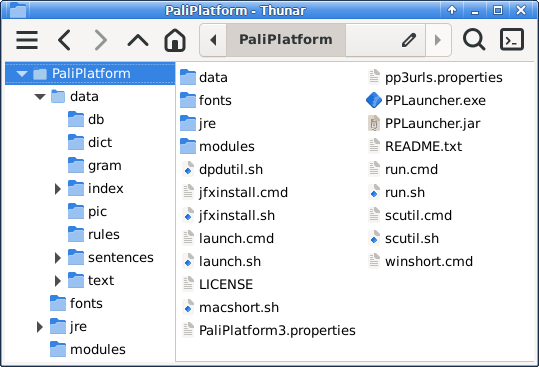
\includegraphics[width=0.9\linewidth]{images/folder-structure.png}\\
\caption{Folder structure of Pāli\,Platform\,3}
\label{fig:folder-structure}
\end{figure}

Note that some files will not appear in your first run, i.e., those ending with \texttt{.properties}, and some directories in \texttt{data} will not be present yet. If you have downloaded the \texttt{winready} package, you will see the \texttt{jre} folder, otherwise you will not. If you see things similar to what is shown above, you are ready to run the program now.

Before that you should examine \texttt{README.txt} with a simple text editor first. This file contains instructions similar to the following sections but in a succinct way, and sometimes it can be more updated. It is also good to know that files ending with \texttt{.cmd} are executable scripts used by Windows machines, and those ending with \texttt{.sh} are used by other OS in the same functionality. These files are essential. Do not delete or modify (if you do not know what you are doing) them.

\subsection{Windows}

The program can run in both 32-bit and 64-bit machines with Windows 7 or newer. I propose several methods described below:

\paragraph{Method 1: Use \texttt{winready} package.} This is the easiest way. After you unpack the package and go into the program's folder, just double-click \texttt{PPLauncher.exe} (the file having the program's logo, in case you do not see the extension). That is all. The only problem that fails the operation is you have downloaded a wrong package. Make sure that you see \texttt{jre} folder before launching the program. After you can make the program start, you can create a desktop launcher by the menu provided.

\newpage
\dothis{With the \texttt{winready} package, the program can be launched simply by double-clicking \texttt{PPLauncher.exe}.}

\paragraph{Method 2: Use your own JRE with JavaFX bundled.} If you have downloaded the normal package, you have to provide JRE to the program yourselves (or you have downloaded the \texttt{winready} package but you want to use another JRE). To make it easy, you should use a JRE bundled with JavaFX. This can be found only in two vendors (Azul and BellSoft). See the links below in the last section. The recent LTS version of Java is recommended. The thing to do here is download a package of this kind, unpack it to the program's root directory, and rename it to `\texttt{jre}.'

\dothis{Once you have obtained a JRE package with JavaFX bundled, unpack it into the program's root directory. Then rename the directory to \texttt{jre}. In case you already have \texttt{jre} folder, delete or rename the old one to something else first. Now you can double-click \texttt{PPLauncher.exe} to start the program.}

\paragraph{Method 3: Use your own JRE.} Another viable solution that is more challenging than the previous one is the use of a JRE without JavaFX. In this case you have to install JavaFX by your own effort, either with the program's installer or with your own hands. For the process of JavaFX installation is similar to all platforms, see Section \ref{sect:javafx-installation} below for details. Once you have JavaFX installed as the program's modules, you can start the program in the same manner as the two previous methods.

\paragraph{Method 4: Use launcher scripts.} This method is for advanced users who are familiar with console terminal. When starting program with \texttt{PPLauncher.exe} seems to fail, this method can be helpful. First, you have to open a terminal (command prompt) at the program's root directory.\footnote{In Windows 10, you can open a terminal at any place in File Explorer by using its \texttt{File} menu.} Then enter \texttt{run} or \texttt{launch} to the prompt. If JVM and JavaFX are present properly, the program will get started.

\dothis{Open a terminal (command prompt) at the program's root directory. Then type this:\\
\commandline[>]{run}\\
or\\
\commandline[>]{launch}
}

Another use case for launching the program with a terminal is to trace the program's bugs when it runs. If you open the program in this way and leave the terminal opened, when the program has errors, it will display messages in the terminal. For advanced users, you may find the causes of the problems. Or better, you can capture the messages and send to the developer together with the symptoms. This can help the developing process considerably.

\boxnote{What's the difference between \texttt{run} and \texttt{launch}?\label{box:run-launch}\\
\hspace{5mm}Both scripts\footnote{In non-Windows machines, these are \texttt{run.sh} and \texttt{launch.sh} respectively. In Windows, \texttt{.cmd} is optional. In most cases, it can be left out.} can make the program start but with a nuance. Technically speaking, \texttt{run} invokes the program's main module directly. If JavaFX is not present, the program will exit with an error. But when \texttt{launch} is used, it invokes \texttt{PPLauncher.jar} instead. Hence, when JavaFX is not present, it will open the installer. Moreover, \texttt{launch} can clean up duplicate modules when patches are applied.\\
\hspace{5mm}This means after a certain update, \texttt{launch} has to be invoked, if not \texttt{PPLauncher.exe}. In Linux and macOS, the program can automatically restart itself after updating, but in Windows it cannot (with an unknown reason). To restart the program properly in this case, use \texttt{PPLauncher.exe} or \texttt{launch} not \texttt{run}.
}

\paragraph{Method 5: Do it a hard way.} This method is unnecessary but it can make you understand the process better. When a JVM is available, you can launch \texttt{PPLauncher.jar} directly as shown below. The effect is equivalent to the use of \texttt{PPLauncher.exe}.

\dothis{Enter this command in a terminal to invoke the program a hard way:\\
\commandline[>]{java -jar PPLauncher.jar}\\
\hspace{5mm}To use \texttt{java} in the \texttt{jre} folder, you have to type this instead:\\
\commandline[>]{jre$\backslash$bin$\backslash$java -jar PPLauncher.jar}
}

\paragraph{Method 6: Do it yet a harder way.} This method is for Java veterans only. It can be used when a JVM and JavaFX are present properly. See the instruction below.

\dothis{Enter this command in a terminal to invoke the program a harder way:\\
\texttt{\small> java -Dfile.encoding=UTF-8 -p "modules"} \neg\\
\hspace{3mm}\texttt{\small-m paliplatform.main/paliplatform.main.PaliPlatform}
}

\subsection{GNU/Linux}

This is my beloved operating system. It fits perfectly with my old/secondhand/cheap computers. Although the number of Linux's users is less than that of Windows and macOS, Linux is a very important OS nowadays. It liberates us. For Linux's users, mostly power users, it looks trivial to tell what to do to run a Java program. So, I will leave out small details.

\paragraph{Step 1: Install Java} If Linux is your day-to-day working environment, it is likely that you have a certain version of Java installed. If its version is 11 or newer, you are done in this step. A simple way to check this is entering `\texttt{java -version}' to a console terminal. If you have none, you have to install one, either by using your Linux distribution's repository\footnote{There is no single right way to do this. It depends on which distribution you use and what kind of package management it uses. Please make familiar with your tools.}, or by downloading one from vendors (see links below) and installing it manually in Java traditional way\footnote{This means you put the acquired JDK/JRE somewhere, set \texttt{JAVA\_HOME} environment, and add its \texttt{bin} directory to the \texttt{PATH}.}. You can also avoid the installation altogether by unpacking the JDK/JRE package into the program's root directory, and rename it to `\texttt{jre}.'

\paragraph{Step 2: Install JavaFX} If Java you have installed in the first step does not have JavaFX combined, you have to install it separately. See further in Section \ref{sect:javafx-installation} below.

\paragraph{Step 3: Use launcher scripts} In the first run, you need a console terminal at the program's root directory to issue a launcher command, either \texttt{run.sh} or \texttt{launch.sh}.\footnote{The difference of the two command is explained in a box note on page \pageref{box:run-launch}.} After the program is active, you can create a desktop launcher for a future use by using the program's menu File.

\dothis{Open a terminal at the program's root directory. Then type this:\\
\commandline{./run.sh}\\
or\\
\commandline{./launch.sh}
}

\paragraph{Optional: Do it a hard way} For power users, you may have a reason to launch the program without any wrapper. Follow the instruction below.

\dothis{To invoke the launcher jar, type this:\\
\commandline{java -jar PPLauncher.jar \&}\\
\hspace{5mm}Or to use \texttt{java} in the \texttt{jre} folder, type this instead:\\
\commandline{jre/bin/java -jar PPLauncher.jar \&}\\
\hspace{5mm}Or to invoke the main module directly, type this:\\
\texttt{\small\$ java -p "modules"} \neg\\
\hspace{3mm}\texttt{\small-m paliplatform.main/paliplatform.main.PaliPlatform \&}
}

\subsection{macOS}

I have never owned or used any of Apple's devices. For the sake of testing, however, I spent many hours to have macOS Catalina (10.15.7) installed in my Linux's virtual machine. So, working on macOS has been tested in a very limited way. The only viable solution to run the program in macOS is using JRE with JavaFX bundled.\footnote{Only two vendors provide this kind of package, namely Azul and BellSoft. See download links below.} (Using a separate JavaFX causes an unexpected termination.) Two choices are available here:

\paragraph{Method 1: Install JRE + JavaFX system-wide (recommended)} When downloading Java, select installation packages with JavaFX included.\footnote{It does not matter whether you use JDK or JRE. For the former choice, you can also develop your own Java programs. For macOS, installation packages are of either \texttt{.pkg} or \texttt{.dmg} files.} Once the installation is successful, you can double-click \texttt{PPLauncher.jar}. Or open a terminal\footnote{In macOS, to open a terminal at a folder, you just simply drag the target folder icon to the Terminal icon on the Dock panel below. Another little harder way is right-clicking the folder icon. Then select Services > New Terminal at Folder.} at the program's root directory and follow Step 3 of the Linux method. After the program works properly, you can create a desktop launcher by the menu provided. This desktop launcher works only the system has Java installed.

\newpage
\boxnote{One problem you may encounter when installing Java to macOS system is that you already have an existing Java without JavaFX. In this case, you have to remove the old Java first. Unfortunately, you must do it manually by opening a terminal and type these commands:\\
\commandline{cd /Library/Java/JavaVirtualMachines}\\
\hspace{5mm}(You do not need to type all of this, just some starters and press Tab.)\\
\commandline{ls}\\
\hspace{5mm}(You will see the list of Java installed, for example in mine, \texttt{liberica-jre-11-full.jre}. If nothing is listed, there is no Java to removed. Then skip the following.)\\
\commandline{sudo rm -rf liberica-jre-11-full.jre}\\
\hspace{5mm}(Do not copy the last part. You have to find out the name on your own.)\\
\hspace{5mm}After the old Java has been removed, a newer one can be installed.
}

\paragraph{Method 2: Install JRE + JavaFX in place} This means you do not want to disturb your system by installing Java. This can be done if you just unpack the Java package you downloaded into the program's root directory (you may choose to download a \texttt{zip} package instead), and rename it to `\texttt{jre}.' Then you can follow Step 3 of the Linux method. One limitation of this solution is that you cannot use the desktop launcher even successfully created.

\section{JavaFX installation}\label{sect:javafx-installation}

JavaFX is a new standard of graphic user interface (GUI) development in Java. Once it was a part of the JDK's library.\footnote{It is still in the library of Java 8.} Now it has a separate line of development. So, to use JavaFX we have to install it properly. The concept is quite simple. You just put the JavaFX \texttt{jar} files in the program's module path. For the platform-dependent side files, you put all of them in the module path as well (in case of Linux and macOS), or you put in directory  \texttt{bin} in the program's root (in case of Windows). Once it is present in the module path, in our case in the directory \texttt{modules}, the program can use it automatically. I will explain two methods of JavaFX installation as follows (remember that to this point a JVM is supposed to be properly installed):

\subsection{Using the internal installer}

To ease the installation, I created a JavaFX installer to use exclusively with the program. If JavaFX is not available, when you invoke the program with \texttt{launch.cmd}, \texttt{launch.sh}, \texttt{PPLaun\-cher.exe}, or \texttt{PPLauncher.jar}, the launcher will lead you to the installer. You can also invoke the installer directly by \texttt{jfxinst\-all.cmd} or \texttt{jfxinstall.sh}.

\dothis{To invoke the JavaFX installer, type this in a terminal opened at the program's root directory, if you use Windows:\\
\commandline[>]{jfxinstall}\\
Or if you use Linux or macOS:\\
\commandline{./jfxinstall.sh}
}

After that you will see a dialog similar to that in Figure \ref{fig:jfxinstall}. The installer will detect your environment and offer you choices to download and install. This depends on what kind of OS you use, what is your machine's architecture, and which version of your Java. The versions of JavaFX available here are predefined. They may not be the latest, but they underwent certain testing.

\begin{figure}[!hbt]
\centering
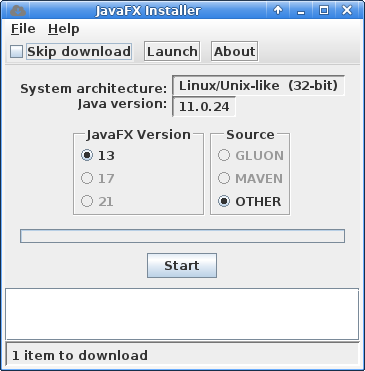
\includegraphics[width=0.8\linewidth]{images/jfxinstall.png}\\
\caption{The JavaFX installer}
\label{fig:jfxinstall}
\end{figure}

If a greater version of JavaFX is available for your environment, it is preferable. And \texttt{Gluon} source, if available, is preferable to \texttt{Maven}.\footnote{Technically speaking, JavaFX modules from the two sources are identical, but they are packaged differently. In the \texttt{Maven} repository, native library files are packed in the modular jars. This is good for portability. For better performance, using packages from \texttt{Gluon} is advisable because the native library is outside the jars.}

After you select a suitable choice, hit the Start button and wait. The installer can launch the program after the installation is finished. Or you may use one of the methods described above. Note that for macOS the installation of independent JavaFX does not work. So, please use a macOS method described above.

\subsection{Installing JavaFX manually}

This method is not recommended but you can do it if you are experienced enough. What you need here is five JavaFX modules, namely \texttt{javafx.base, javafx.controls, javafx.graphics, javafx.media,} and \texttt{javafx.web}. If you download these from Maven repository, just put these jar files into directory \texttt{modules} of the program. All existing JavaFX jars have be removed first. That is a good thing about Maven's packages.

In case you download JavaFX packages from Gluon, normally in one zip file, you have to unpack it somewhere first. Then copy everything in directory \texttt{lib} to the program's \texttt{modules}. For Windows, you will also see directory named \texttt{bin}. Copy the whole directory to the program's root. This means now the root directory of the program will have \texttt{bin} with its content. Any existing JavaFX components have to be removed before copying.

\section{When things go right}

Once you succeed to make the program run in your computer, you will see the main window as shown in Figure \ref{fig:main-window}. In each tab, you will see a Load button at first. Click it to load the content of the tabs. This has to be done once in each start. This strategy can reduce the starting time of the program.

\begin{figure}[!hbt]
\centering
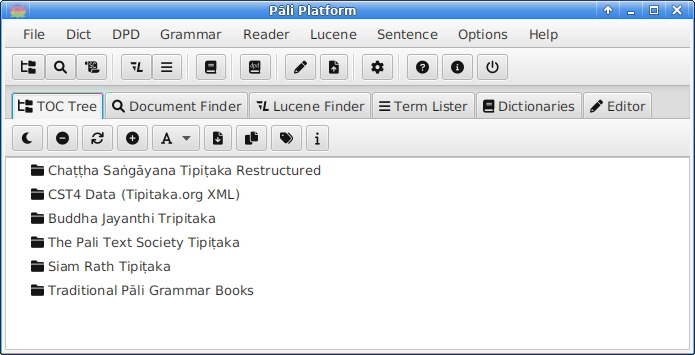
\includegraphics[width=0.9\linewidth]{images/main-window.png}\\
\caption{Main window of \textsc{Pāli\,Platform\,3}}
\label{fig:main-window}
\end{figure}

After you see the main window, it is better to see the program's About by choosing Help > About in the menu, or clicking {\faSix \symbol{"F05A}} button. On the left of the dialog, your system's information will be shown (see Figure \ref{fig:about}). Your information should be different from mine. There is a gimmick hidden in this About window. Find it if you are curious.

\begin{figure}[!hbt]
\centering
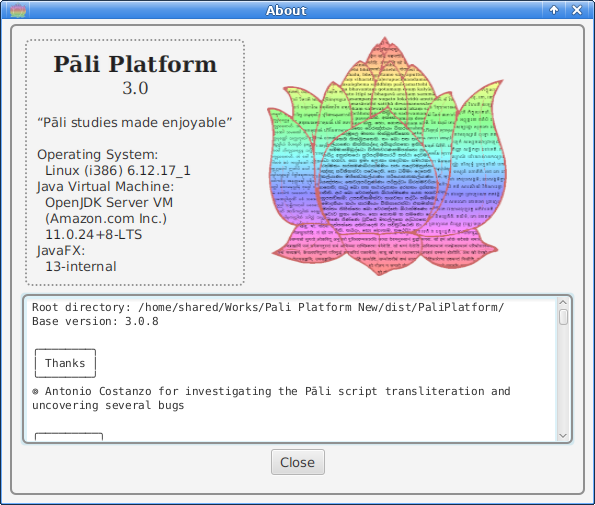
\includegraphics[width=0.9\linewidth]{images/about.png}\\
\caption{About window}
\label{fig:about}
\end{figure}

\section{When things go wrong}

Even though the program was somewhat well-tested, many bugs are still waiting. They can show up when encountering unexpected use cases that are overlooked in testing. To trace the cause of errors, you have to run the program with a terminal and leave it opened. When the program crashes, error messages will show up in the terminal. A simple example is shown in the box below.

\boxnote{Here is the error message when the program starts without JavaFX:\\
\commandline{./run.sh}\\
\texttt{\small Error occurred during initialization of boot layer}\\
\texttt{\small java.lang.module.FindException: Module javafx.base not found, required by paliplatform.main}
}

Error messages can be very complicated in some critical cases. If the users find that the program behaves in an unusual way or even crashes unexpectedly, please start it again with a terminal and do the same thing as before. The messages will tell you the causes. If they are intelligible, capture the messages and report the bugs to the developer.

\section{Related download links}

Here are some useful links related to the program's execution. If possible, use a JRE of recent LTS Java (Java 17 and 21 are normally faster than 11).

\paragraph{(1) Azul Zulu JDK.} Azul Systems provides JRE with JavaFX (32-bit and 64-bit) for many platforms, but few have installers. When downloading, select JRE FX.

\begin{compactitem}
\item \url{www.azul.com/downloads/?package=jdk#zulu}
\end{compactitem}

\paragraph{(2) BellSoft Liberica JDK.} BellSoft also provides installers of JRE with JavaFX for major platforms. This can be easy for new users who just want to install what is needed. When downloading, select JRE Full.

\begin{compactitem}
\item \url{bell-sw.com/pages/downloads}
\end{compactitem}

\paragraph{(3) Eclipse Temurin JDK.} This provider does not have JavaFX, just JRE. This may be suitable for a competent user who knows how to combine the two components together (see the instructions above).

\begin{compactitem}
\item \url{adoptium.net/temurin}
\end{compactitem}


\paragraph{(4) Gluon's JavaFX.} This is the official site of JavaFX. You rarely need this, except if you want the newest version of it (really unnecessary for us). When downloading, select SDK binary package, not \texttt{jmods}.

\begin{compactitem}
\item \url{gluonhq.com/products/javafx}
\end{compactitem}



